\section{Results}
\label{sec:results}

\begin{figure}[t]
  \centering
  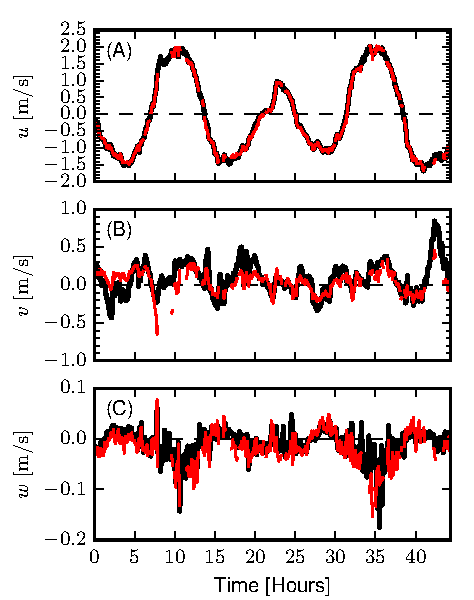
\includegraphics{TimeFig02}
  \caption{Time series of tidal velocity in June 2012 at Admiralty Head from ADV-IMU measurements (black), and an ADP on the anchor (red). Note that the vertical scale on the three axes vary by an order of magnitude; the small ticks in A and B are equivalent to the ticks in C.}
  \label{fig:vel_time}
\end{figure}

\subsection{Mean velocity}

Figure \ref{fig:vel_time} shows a comparison of $\vec{\bar u}$ measured by an ADV-IMU mounted on the TTM, to an upward-looking ADP on the anchor. The profiler measurements---taken at the same depth as the ADV on the TTM---were contaminated by acoustic reflection from the strongback fin when it was inline with one of the profiler's beams (see section \ref{sec:meas}.\ref{sec:meas:ttm}). When those points (not shown in the figure) are excluded, this comparison shows excellent agreement between the ADV and ADP measurements of mean velocity. The $\bar u$, $\bar v$, and $\bar w$ components have a root-mean-square error of 0.05, 0.13, and 0.03 ms$^{-1}$, respectively. Although it is important to note that there is some discrepancy between ADP- and ADV-measured velocities (especially in $\bar v$, which is most likely due to incomplete motion correction), the agreement between the magnitude and direction of these independent velocity measurements indicates that moored ADV-IMUs provide a reliable estimate of mean velocity in the Earth's reference frame.

\subsection{TTM spectra}

\begin{figure*}[t]
  \centering
  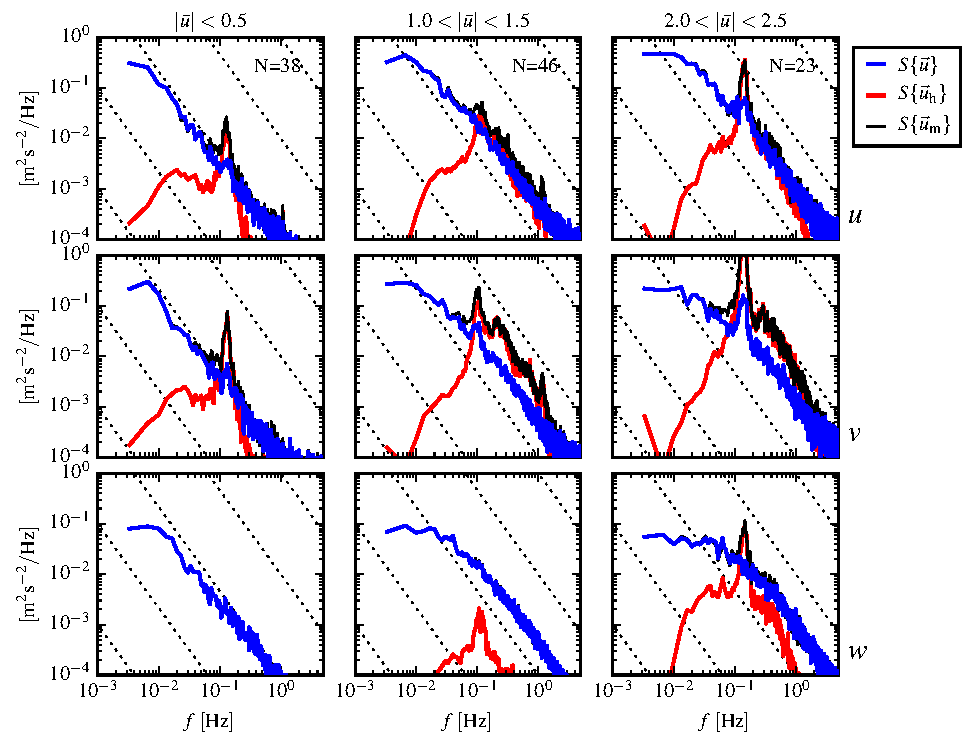
\includegraphics{SpecFig02_TTM02B-top}
  \caption{Turbulence spectra from the June 2014 TTM deployment. Each column is for a range of streamwise velocity magnitudes (indicated at top, in $\mathrm{m\,s^{-1}}$). The rows are for each component of velocity (indicated at far right). The uncorrected spectra are black, the corrected spectra are blue, and the spectra of ADV head motion is red (also indicated in the legend). The vertical red dotted line indicates $f_a$ for estimating $\uhead$; below this frequency $\spec{\uhead}$ is plotted as a dashed line.   Diagonal black dotted lines indicate a $f^{-5/3}$ slope. The cyan line in the first and last rows indicates the semi-empirical Kaimal spectrum for the measured values of $\ustar$ and $\bar U$. The number of spectral ensembles, N, in each column is indicated in the top row.}
  \label{fig:spec:ttm}
\end{figure*}

As discussed in detail in Part 1, the mooring motion of the TTM, $\spec{\uhead}$, has a peak at 0.1 to 0.2 Hz from swaying of the mooring that is most likely driven by eddy shedding from the spherical buoy (Figure \ref{fig:spec:ttm}, red lines). There is also higher-frequency broadband motion that is associated with fluttering of the strongback fin around the mooring line. These motions are especially energetic in $\spec{v}$ because this is the direction in which the TTM is most unstable. As is expected from fluid-structure interaction theory, the amplitude of these motions increases with increasing mean velocity \cite[]{Morison++1950}.

The mooring motion contaminates the uncorrected ADV measurements of velocity, $\spec{\umeas}$, whenever the amplitude of the motion is similar to or greater than the amplitude of the turbulence. Fortunately, much of this motion can be removed as detailed in Section \ref{sec:methods}. At high frequencies ($f>0.3$ Hz) for each mean-flow speed $\spec{\ue}$ are consistent with \citeauthor{Kolmogorov1941c}'s (1941) theory of isotropic turbulence: the spectra decay with a $f^{-5/3}$ slope and have equal amplitude across the velocity components. At lower frequencies, the spectral `roll-off' shape is similar to that measured by several others \cite[e.g.,][]{Thomson++2012, McMillan++2016}. The degree of agreement between \citeauthor{Kaimal++1972}'s (1972) semi-empirical form (cyan) and $\spec{\ue}$ is similar to that of \cite{Walter++2011}. This suggests that bottom-boundary layer physics are contributing to the turbulence at this site and depth.

For $|\ue|>1.0$ ms$^{-1}$, motion correction improves $\spec{u}$ and $\spec{v}$ at frequencies as high as 3 Hz. This indicates that tight synchronization between the ADV and IMU is important and that implementing asynchronous approaches to motion correction may be challenging.

As successful as motion correction is, some motion contamination is `persistent'. This is most notable in $\spec{v}$ at the highest flow speeds ($>2.0$ ms$^{-1}$): a peak at 0.15 Hz is an order of magnitude larger than a smooth spectral shape would suggest. This persistent motion contamination is evident to a lesser degree in $\spec{u}$ for $|u|>2$ ms$^{-1}$, and in $\spec{v}$ at lower flow speeds.  $\spec{w}$ appears to have no persistent motion contamination because the amplitude of the motion in this direction is much lower than the measured spectra.

The amplitude of the persistent motion contamination peaks in $\spec{v}$ at 0.15 Hz is a factor of 5 to 10 times smaller than the amplitude of the ADV head motion itself. This observation suggests that the Microstrain IMU can be used to effectively correct mooring motion at this frequency when the amplitude of that motion is less than 5 times the amplitude of the real turbulence spectrum. As a result, we have chosen a value of 3 as a conservative estimate of motion correction's effectiveness.

In addition to the primary benefit of correcting for mooring motion, the IMU measurements can also be used to identify and screen out persistent motion contamination. For example, one of the most common uses of turbulence spectra is for the calculation of $\epsilon$ and $\tke$. For these purposes, and based on the relative amplitudes of the 0.15-Hz peaks, we assume that persistent motion contamination is likely where $\spec{\uhead}/\spec{\ue} > 3$, and thereby exclude these regions from spectral fits.

In the present case, for $u$- and $w$-component spectra, this criteria only excludes a narrow range of frequencies at the 0.15-Hz motion peak for the largest flow speeds. This criteria is more restrictive of $v$-component spectra at high frequencies for $\bar U > 1.0$ ms$^{-1}$, but this may be acceptable because the amplitude of $\spec{v}$ at these frequencies---i.e., in the isotropic inertial subrange---should be equal to that of $\spec{u}$ and $\spec{w}$ \cite[]{Kolmogorov1941c}.

Agreement of $\spec{v}$ with that of $\spec{u}$ and $\spec{w}$ at frequencies $>0.3$ Hz indicates that motion correction is effective at those frequencies even when $\spec{\uhead}/\spec{\ue} \gtrsim 3$. This outcome suggests that our screening threshold is excessively conservative at those frequencies, and that a more precise screening threshold may be frequency dependent. For example, it might take into account the $~f^{-2}$ character of the noise in $\spec{\uacc}$ (Figure \ref{fig:stnoise}). For the purpose of this work, the $\spec{\uhead}/\spec{\ue} < 3$ threshold for spectral fits is sufficient, and detailed characterization of the IMU's motion- and frequency-dependent noise level is left for future work.

\subsection{StableMoor Spectra}

\begin{figure*}[th]
  \centering
  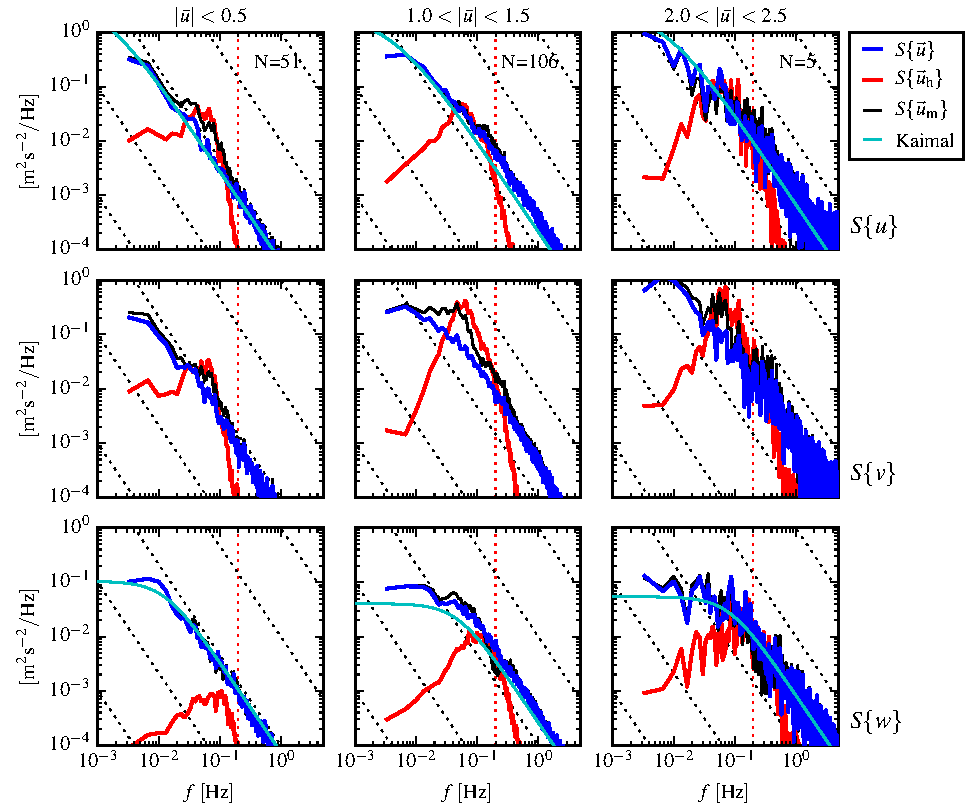
\includegraphics{SpecFig02_SMnose}
  \caption{Turbulence spectra from the SMB. The axes layout and annotations are identical to Figure \ref{fig:spec:ttm}, except that $\spec{\uhead}$ is plotted as a solid line at all frequencies because it is measured at all frequencies. }
  \label{fig:spec:sm}
\end{figure*}

Spectra of SMB motion have broader peaks, with a maximum amplitude that is approximately half the frequency of the TTM spectral peak (0.06 Hz, Figure \ref{fig:spec:sm}). The motion of this platform also does not have high-frequency ``subpeaks" or other high-frequency broadband excitation (Part 1).  These characteristics are due to the more massive and hydrodynamically streamlined properties of the SMB compared to the TTM. 

Like the TTM, the motion-corrected spectra from the SMB are consistent with turbulence theory and previous observations. A notable distinction from the TTM, however, is that there are no obvious persistent motion contamination peaks. That is, this measurement system provides an accurate estimate of the turbulence spectra at this location from low frequencies to more than 1 Hz---well into the inertial subrange---for all three components of velocity.

Note that this level of accuracy cannot be obtained without the independent estimate of $\ulow$ (from the bottom-tracking ADP). If we assume that $\ulow=0$, a similar plot to Figure \ref{fig:spec:sm} (not shown) reveals persistent motion-contamination peaks and troughs in $\spec{u}$ and $\spec{v}$ regardless of the choice of $f_a$. This indicates that the low-frequency translational motion of the SMB that is important to motion correction is poorly resolved by the IMU's accelerometer. In other words, compared to the TTM, the SMB provides a more accurate measurement of turbulence when it includes an independent measure of $\ulow$, but it does no better---and perhaps worse---when it does not.

\subsection{Torpedo spectra}

\begin{figure}[t]
  \centering
  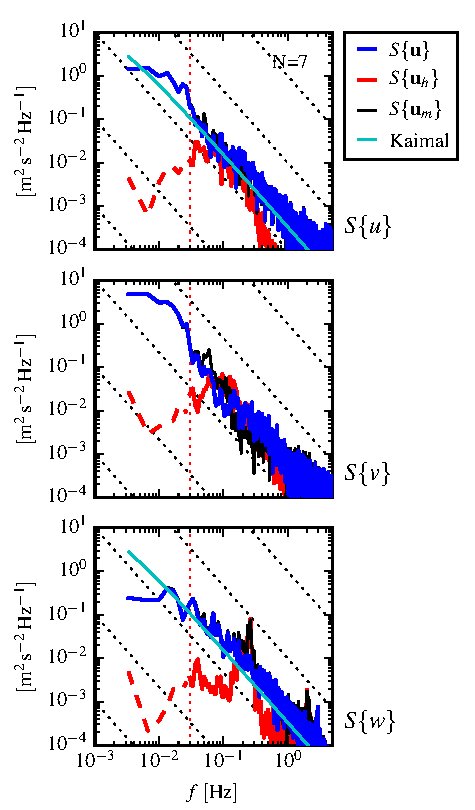
\includegraphics{SpecFig03_TTT}
  \caption{Turbulence spectra from the turbulence torpedo during a 35-minute period when the mean velocity was 1.3 $\mathrm{m\,s^{-1}}$. Annotations and line colors are identical to Figure \ref{fig:spec:ttm}.}
  \label{fig:spec:torpedo}
\end{figure}

$\spec{u_\head}$ and $\spec{v_\head}$ for the turbulence torpedo is broadband and $\spec{w_\head}$ motion has a narrow peak at 0.3 Hz (Figure \ref{fig:spec:torpedo}). Because $\uhead$ is estimated using $f_a = 0.03$ Hz and assuming $\ulow=0$, its spectra rolls off quickly below $f_a$.  Motion correction of the torpedo data appears to effectively remove a motion peak from $\spec{w}$ at 0.3 Hz, and corrects $\spec{v}$ between 0.04 and 0.6 Hz. $\spec{u}$ is mostly unaffected by motion at these frequencies, because the torpedo motion is smaller than the turbulence in this direction. At frequencies below $f_a$, $\spec{u}$ and $\spec{v}$ increase dramatically. This suggests that unresolved, low-frequency motion of the torpedo is contaminating the velocity measurements at these frequencies. It may be possible to correct for some of this contamination using a measurement of the ship's motion as a proxy for the torpedo's low-frequency motion, but this has not been done. Still, above $f_a$, the torpedo appears to provide a reliable estimate of spectral amplitude in the inertial subrange and can therefore be used to estimate $\epsilon$. Considering the simplicity of the platform, it may be a useful option for quantifying this turbulence statistic in a variety of scenarios. If a GPS is positioned above it, it may be capable of providing even more.


\subsection{Cross Spectra}

\begin{figure}[t]
  \centering
  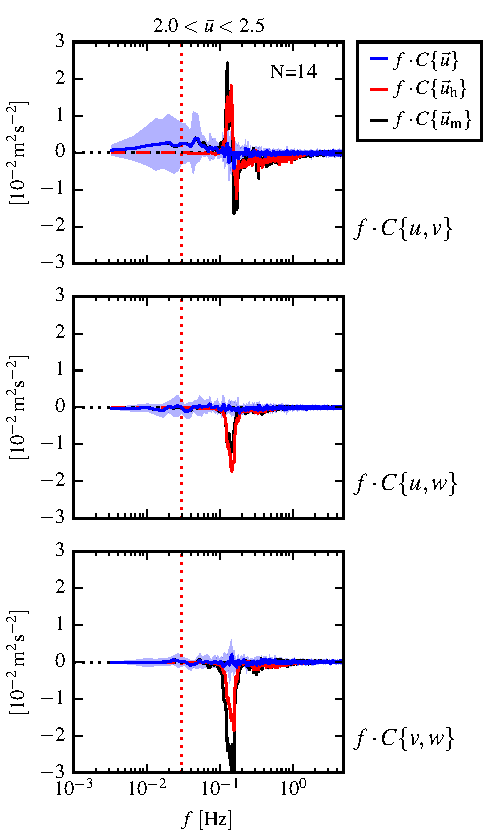
\includegraphics{StressSpec_TTM_04vp}
  \caption{Variance preserving cross-spectra between components of $\ue$ (blue), $\uhead$ (red), and $\umeas$ (black) from the June 2014 TTM deployment. The upper row is $f\,\cspec{u}{v}$, the middle row is $f\,\cspec{u}{w}$, and the bottom row is $f\,\cspec{v}{w}$ (also indicated at right).  Note that these cross-spectra are between components of a velocity vector (e.g., $\ue$), not between different vectors (i.e., not between $\ue$ and $\umeas$). N is the number of spectral ensembles in this average, i.e. when $2 < |u| < 2.5\,\mathrm{m\,s^{-1}}$. The light blue shading indicates one standard deviation of $f\,C\{\ue\}$.}
  \label{fig:cspec:ttm}
\end{figure}

Cross-spectra indicate the correlation between different velocity components as a function of frequency, and their integrals are the Reynold's stresses. Head motion cross-spectra, $C\{\uhead\}$ (Figure \ref{fig:cspec:ttm}, red), and uncorrected velocity cross-spectra, $C\lbrace \umeas \rbrace$ (black), from TTM measurements have large peaks at the same frequency (0.15 Hz) as peaks in auto-spectra (Figure \ref{fig:spec:ttm}).  This indicates that mooring motion contaminates the uncorrected cross-spectral velocity measurements, and that Reynold's stress estimates based on uncorrected velocity measurements will be contaminated by mooring motion. 

Fortunately, motion corrected velocity cross-spectra, $C\{\ue\}$ (Figure \ref{fig:cspec:ttm}, blue), have reduced cross-spectral amplitudes at these frequencies. This indicates that motion correction reduces motion contamination to produce more reliable estimates of velocity cross spectra and Reynold's stresses (Figure \ref{fig:cspec:ttm}). Notably, the low standard deviation of $f\, C\{\ue\}$ (indicated by the blue shading) compared to the mean values of $f\,C\{\uhead\}$ and $f\,C\{\umeas\}$---at the frequencies of maximum motion---indicates that even the individual values of $C\{\ue\}$ are reduced at these frequencies, compared to $C\{\umeas\}$, not just their mean.

These results indicate that motion-corrected TTM velocity measurements can be used to estimate turbulence Reynold's stresses. Without motion correction, Reynold's stress estimates would be contaminated by the large peaks in the cross spectra that are caused by the swaying and fluttering motion of the TTM vane. Cross-spectra of TTM data for other velocity ranges (i.e., $<$ 2 ms$^{-1}$), and cross-spectra from the SMB show similar results (not shown). However, we note that because the SMB is less-stable in pitch than the TTM (see Part I for details), the TTM provides a more accurate estimates of  $\uw$.

\begin{figure}[t]
  \centering
  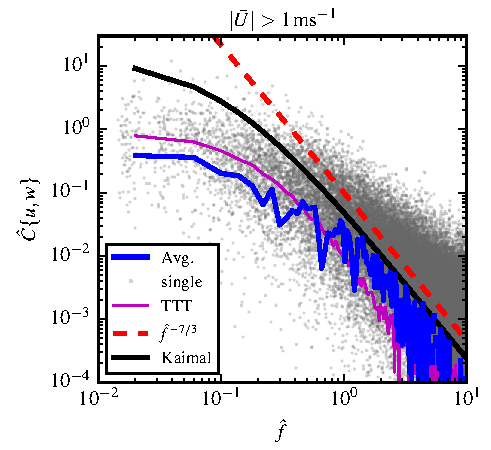
\includegraphics{CoSpecND03_TTM-both}
  \caption{Non-dimensional cross-spectra of motion corrected velocity, $\hat{C}\{u,w\}$, on a log-log scale. The average over $\Delta \hat{f} = 0.04$ bins is shown in blue, and single points are grey (negative values not shown). The semi-empirical \cite{Kaimal++1972} form is shown as a thick black line, and the red dashed line indicates a $\hat{f}^{-7/3}$ slope. Cross-spectral estimates from measurements from a fixed `tripod' are in purple.}
  \label{fig:cspecnd:ttm}
\end{figure}

In order to compare the cross-spectra to other measurements, we normalize them following \cite{Kaimal++1972} as: $\hat{C}\{u,w\}(\hat{f}) = -\cspec{u}{w} f_\circ / \ustar^2$, where $f_\circ = \bar{U} / z$ and $\hat{f} = f / f_\circ$. 
When plotted on a log-log scale, $\hat{C}\lbrace u,w \rbrace$ has a $\hat{f}^{-7/3}$ high-frequency spectral slope that is consistent with other measurements (Figure \ref{fig:cspecnd:ttm}). At low-frequency, the cross-spectra are more than 10x smaller than the semi-empirical Kaimal form, but this discrepancy is consistent with other measurements of cross-spectra. In particular, \cite{Walter++2011} observed a half-decade reduction from the Kaimal form near the seafloor, and measurements from an ADV positioned 4.6 m above the seafloor on a fixed tripod at a different site in Puget Sound show a similar degree of deviation as observed here \cite[]{Thomson++2012}. 

While one might be inclined to attribute the discrepancy between these estimates and the Kaimal form to normalization by local $\ustar$, the agreement between auto-spectra and their Kaimal form suggests otherwise (Figure \ref{fig:spec:ttm}). Instead, we conclude that either the Kaimal cross-spectra do not apply universally at distances far from the bottom boundary, or the spectra are being modified by physics other than bottom boundary layer driven turbulence. Either way, the agreement of TTM-measured cross-spectra with measurements from stationary platforms is interpreted as an indication that this platform can resolve cross-spectra and Reynold's stresses.

%%% Local Variables:
%%% mode: latex
%%% TeX-master: "Kilcher_etal_IMU-ADV"
%%% End:
